\documentclass[xcolor=dvipsnames,slidestop,compress,mathserif,color]{beamer}
\usepackage[english,spanish]{babel}
\usepackage[utf8]{inputenc}
\usepackage{listings}
\usepackage[noend]{algorithmic}

\useoutertheme[subsection=false,footline=authortitle]{miniframes}
\useinnertheme[shadow]{rounded}
\usecolortheme{orchid}
\setbeamercolor{separation line}{use=structure,bg=structure.fg!50!bg}

\logo{
\includegraphics[height=1cm]{../images/logo_inf}}

\title{Extracción de superficies a partir de una colección de puntos en un dominio tridimensional}
\author{Joe Cabezas}

\institute[UTFSM]{
Departamento de Inform\'atica\\
Universidad T\'ecnica Federico Santa Mar\'ia}
\date[ICI]{\tiny{Thesis Presented in Partial Fulfillment of the Requirements
for the Engineering Degree}\\ \Large{Ingeniero Civil en Inform\'atica}}

\makeindex

\newenvironment<>{varblock}[2][\textwidth]{%
	\setlength{\textwidth}{#1}
	\begin{actionenv}#3%
		\def\insertblocktitle{#2}%
		\par%
		\usebeamertemplate{block begin}}
	{\par%
		\usebeamertemplate{block end}%
	\end{actionenv}}

\begin{document}

\begin{frame}
\titlepage
\end{frame}

\begin{frame}
	\frametitle{Contenido}
	\tableofcontents
	%\tableofcontents[currentsection,currentsubsection]
	%\begin{columns}
	%\begin{column}{0.5\textwidth}
	%\tableofcontents[sections={1-3}]
	%\end{column}
	%\begin{column}{0.5\textwidth}
	%\tableofcontents[sections={4-8}]
	%\end{column}
	%\end{columns}
\end{frame}

\section{Introducción}

\begin{frame}
\frametitle{Introducción}
	\begin{block}{}
		\begin{itemize}[<+->]
			\item Mallas Geométricas.
			\item Uso de las Mallas Geométricas.
			\item Consideraciones Físicas.
			\item Objetivos.
		\end{itemize}
	\end{block}
\end{frame}

\subsection{Mallas Geométricas}

\begin{frame}
\frametitle{Mallas Geométricas}

\only<1>
{
	%\begin{block}{Mallas Geométricas}
		\begin{itemize}
			\item Conjunto de polígonos (triángulos, cuadriláteros, etc.),
						que conforman una superficie en un espacio definido.
			\item Las mallas tienen asociadas un conjunto de
						elementos topológicos tales como: vértices, aristas, y caras poligonales.
			\item Describen regiones en un plano, volumenes en un espacio.
			\item Realizar esta discretización consiste en
aproximar el dominio a simular dividiéndolo en elementos geométricos mas sencillos.
		\end{itemize}
	%\end{block}
		\begin{figure}
			\center
				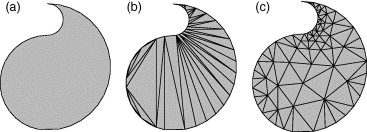
\includegraphics[width=0.55\textwidth]{images/introduction/triangulation.jpg}
		\end{figure}
}
\only<2>
{
	\begin{itemize}
		\item Ejemplo 3D
	\end{itemize}
	\begin{figure}
		\center
			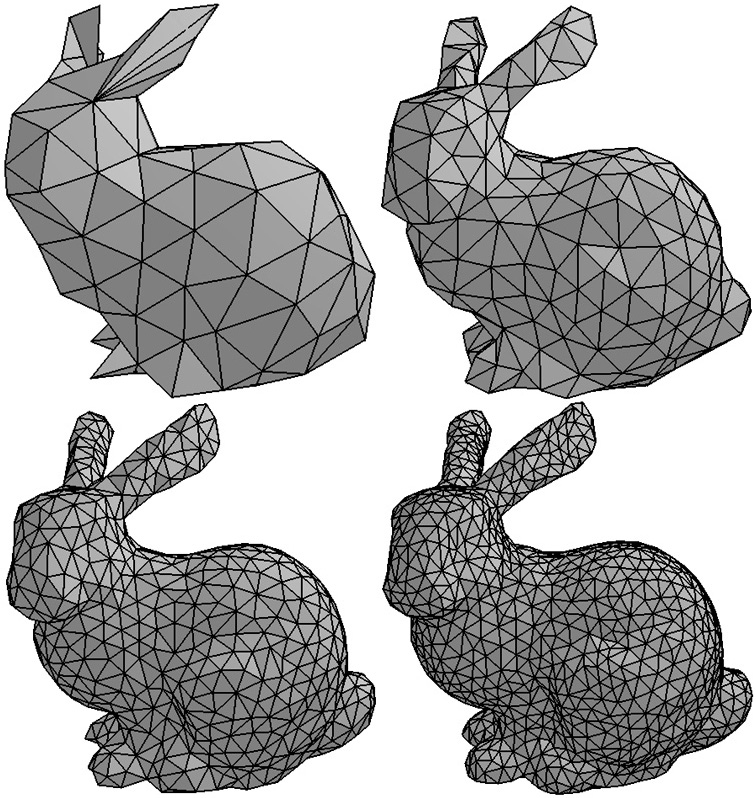
\includegraphics[width=0.5\textwidth]{images/introduction/mesh_remeshing2.jpg}
	\end{figure}
}
\end{frame}

\subsection{Usos de las Mallas Geométricas}

\begin{frame}
\frametitle{Usos de las Mallas Geométricas}
	\begin{block}<1->{Simulaciones físicas}
		\begin{itemize}[<+->]
			\item Estudio de fuerzas.
			\item Interaccion de objetos.
			\item Simulacion de fluidos.
		\end{itemize}
	\end{block}
	\begin{block}<4->{Gráficos}
		\begin{itemize}[<+->]
			\item Visualización de cuerpos en tres dimensiones.
			\item Visualización de funciones matemáticas.
		\end{itemize}
	\end{block}
	\begin{varblock}[0.9\textwidth]{Artísticos}<6->
		\begin{itemize}[<+->]
			\item Gráficos realistas.
			\item Animación.
			\item Películas.
		\end{itemize}
	\end{varblock}
\end{frame}


\subsection{Consideraciones Físicas}
\begin{frame}
	\frametitle{Consideraciones Físicas}
	\begin{itemize}[<+->]
		\item Vivimos en un mundo en tres dimensiones.
			\begin{itemize}
				\item Posición específica dentro de un espacio continuo.
				\item No existe una distancia mínima para el desplazamiento.
			\end{itemize}
		\item La continuidad representa un problema en el mundo virtual.
		\item Los objetos estan compuestos de materia.
			\begin{itemize}
				\item Los objetos en el mundo vitual no están (ni pueden aún) ser
							descritos por unidades atómicas.
			\end{itemize}
		\item Los objetos en el mundo virtual son representados por una cantidad discreta
					de triángulos, formando una superficie.
		\item Simples discretizaciones de los objetos reales, sin propiedades físicas como el roce.
			\begin{itemize}
				\item Mesa infinitamente lisa.
			\end{itemize}
	\end{itemize}
\end{frame}

\subsection{Objetos en tres dimensiones}
\begin{frame}
	\frametitle{Objetos en tres dimensiones}
	\begin{itemize}[<+->]
		\item Conjunto de planos triangulares que forman la superficie externa y visible del objeto.
		\item Para extraer la información de la forma de un objeto existen diversas tecnologías.
			\begin{itemize}
				\item Software capaz de generar modelos usando arreglo de fotografías.
				\item Arreglo de cámaras que capturan en tiempo real una nube de puntos infrarrojos.
				\item Equipos de imagenología de resonancia magnética.
					\begin{itemize}
						\item Técnica no invasiva que utiliza el fenómeno de la resonancia magnética, obtiene
									información de la estructura y composición del cuerpo a analizar.
						\item La información obtenida procesada por un software que genera una malla
									geométrica del área de interés
						\item ;)
					\end{itemize}
			\end{itemize}
	\end{itemize}
\end{frame}

\subsection{Objetivos}
\begin{frame}
	\frametitle{Objetivos}
	\begin{itemize}[<+->]
		\item Se propondrá un flujo de trabajo que permita la extracción de una superficie
					dada una colección de puntos en un espacio tridimensional.
			\begin{itemize}
				\item Se hará énfasis en los primeros pasos del flujo propuesto.
			\end{itemize}
		\item Para ello se estudiará el algoritmo de \emph{Marching Cubes}.
			\begin{itemize}
				\item Hacer la extracción de una malla de superficie.
			\end{itemize}
		\item Se construirá una herramienta de visualización y navegación que ayudará a la correcta
					elección del valor mínimo para poder extraer una superficie con un nivel de detalle controlable por el investigador.
	\end{itemize}
\end{frame}

\section{Estado del Arte}

\begin{frame}
\frametitle{Solution Requirements}
\begin{block}{Design}<1->
\begin{itemize}
\item Model Driven Generation
\end{itemize}
\end{block}
\only<1>{
%\begin{figure}
%\includegraphics[width=0.7\textwidth]{MARS-classdiagram-full}
%\end{figure}
}
\only<2>{
%\begin{figure}
%\includegraphics[width=0.7\textwidth]{MARS-zoom}
%\end{figure}
}
\only<3>{
%\begin{figure}
%\includegraphics[height=0.65\textheight]{general-workflow}
%\end{figure}
}
\end{frame}
\subsection[Design]{Solution Design}
\begin{frame}
\begin{varblock}[0.9\textwidth]{How is it done?}
%\begin{center}
%\includegraphics[height=0.68\textwidth]{design}
%\end{center}
\end{varblock}
\end{frame}

\begin{frame}[fragile]
\begin{varblock}[0.9\textwidth]{Template}
\begin{verbatim}
«IMPORT uml»
«EXTENSION templates::util»

«DEFINE Root FOR uml::Model»
«FILE 'idl/'+this.name+"Common.idl"»
#ifndef «this.name»_IDL
#define «this.name»_IDL
#pragma prefix "alma"

module «this.name»
{
«FOREACH allOwnedElements().
			typeSelect(uml::Enumeration) AS element»
				«EXPAND ENUM FOR element»
«ENDFOREACH-»
\end{verbatim}
\end{varblock}
\end{frame}
\begin{frame}[fragile]
\begin{varblock}[0.9\textwidth]{Template}
\begin{verbatim}
«DEFINE ENUM FOR uml::Enumeration»
		enum «this.name» {
		«FOREACH  this.eAllContents.
					typeSelect(uml::EnumerationLiteral)
									 AS element SEPARATOR ', '»
							 «element.name»
				«ENDFOREACH»
		};
«ENDDEFINE»
\end{verbatim}
\end{varblock}
\end{frame}
\subsection[Separation]{Isolating the complexity}
\begin{frame}
\begin{varblock}[0.9\textwidth]{Code Separation}
%\begin{center}
%\includegraphics[width=0.85\textwidth]{separation}
%\end{center}
\only<2>{
\centering
\textbf{Keep generated code clear from hand crafted code.}
}
\end{varblock}
\end{frame}


\section[Future]{Future Work}
\begin{frame}
\vspace{2cm}
\begin{block}{Author's Comment}
The biggest contribution of this work
is the possibilities and future work it has created.
\end{block}

\end{frame}
\subsection[Basic]{Basic Extension}
\begin{frame}
	 \frametitle{Future Work}
\begin{block}{Inmediate Extensions}
\begin{itemize}
	 \item Support for \texttt{C++} and \texttt{Python}.
	 \item Flexible package definition.
	 \item Inheritance support between genereted and non generated code.
	 \item Model checking usign OAW Check facility.
	 \item Implement exceptions definition support.
	 \item integrate the generation process with the ACS build process.
\end{itemize}
\end{block}
\end{frame}
\subsection[Advanced]{Advanced Extension}
\begin{frame}
	 \frametitle{Future Work}
\begin{block}{Advanced Extensions}
\begin{itemize}
	 \item Integrate with the ACS state machine generator.
	 \item Merge work done in the ACS genertaor and bdsGenerator.
	 \item Enable static resource definition.
	 \item Provide a full type profile to avoid stereotypes.
	 \item Identify common coding patterns in the implemented code
				 and move the to the templates.
\end{itemize}
\end{block}
\end{frame}
\section[Appendix]{Appendix}
\begin{frame}
	 \frametitle{Published Papers}
	 \begin{itemize}
			\item \textit{{ALMA} {Common} {Software} {(ACS)}, Status and Development},
			\mbox{G. Chiozzi} et al.,
			\textbf{Proceedings of ICALEPS}, October 2009.
			\item A second publication in the making,
			to be presented on the call for papers of the \textbf{SPIE}, 2010.
	 \end{itemize}
\end{frame}
%\subsection[]{}
%\subsection[]{}

\section*{End}
\begin{frame}
\frametitle{Questions?}
\begin{center}
\end{center}
\end{frame}

\end{document}

